\documentclass[12pt]{article}
\usepackage{amssymb}
\usepackage[UTF8]{ctex}
\usepackage{geometry}
\usepackage{units}
\usepackage{pifont}
\geometry{
	a4paper,
	total={150mm,237mm},
	left=30mm,
	top=27mm,
	}
\usepackage{amsmath}
\usepackage{enumerate}
\usepackage{lipsum}
\usepackage{graphicx}
\usepackage{hyperref}
\usepackage{indentfirst}
\usepackage[graphicx]{realboxes}
\usepackage{booktabs}
\usepackage{cases}
\usepackage{subfig}  
\usepackage{float}
\usepackage{xcolor}
\setlength{\parindent}{2em}
\title{Lab4}
\author{姓名:陈锐林,学号:21307130148}
\date{\today}

\begin{document}
\maketitle
\begin{Large}
	\noindent 实验1:RISCV-实验\\
\end{Large}
Question-1:\par
(1)根据参考资料可知,RISCV中,函数参数保存在寄存器a0-a7中。(2)如这里main中的参数13,应该是保存在a2中;因为有这么一句
"li a2,13"。\\
Question-2:\par
可以看到,因为系统内联了函数,所以在main的汇编代码中并没有明确调用。这里要计算f(8)+3,能看到,这里是直接"li a1,12",进行了赋值。
\begin{figure}[H]
    \centering
    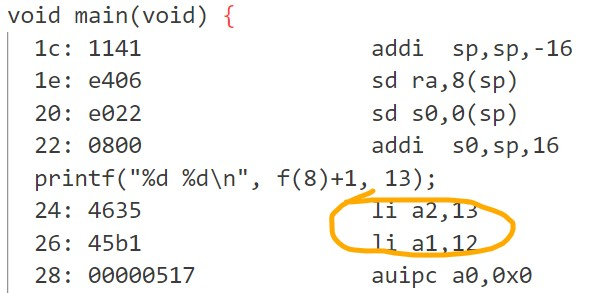
\includegraphics[height=4cm,width=6.5cm]{lab4-1.jpg}
\end{figure}
\noindent Question-3:\par
主要是下面两行代码。auipc这行就是把pc+(常数>>12)给ra;下一行就是跳转到地址为1554+ra的地方,即printf。所以这里printf的地址就是这个结果0x0000000000000642。
\begin{figure}[H]
    \centering
    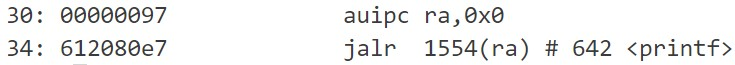
\includegraphics[height=1.5cm,width=6.5cm]{lab4-2.jpg}
\end{figure}
\noindent Question-4:\par
ra应该保存函数返回地址,即38。
\newpage
\noindent Question-5:\par
这里57616即0xe110,\%x即直接以16进制输出。(1)按小端执行,i的内部储存为"0x726c6400",\%输出字符串,再根据ASCII码表,每两位一输出;最后结果是"He110,World\textbackslash{}0"。
(2)如果改成大端法表示,57616无需修改,因为还是16进制输出;而需要对i进行翻转,unsigned int i = 0x726c6400。\\
Question-6:\par
多次运行,会看到输出的值不同。联系1中内容可以知道,这时候printf需要两个参数,第一个参数给出为3,但是第二个未知;这时候应该直接输出a2中的值。\\

\begin{Large}
	\noindent 实验2:Backtrace实验\\
\end{Large}
1.思路如下:\par
由参考资料的这个图能看出来,函数的调用栈是这么个结构(可递归自底向上)。假设我们知道最底部的fp,那么首先可以根据fp-8得到这个函数的返回地址ra;还能知道上一个函数栈的fp储存在地址为fp-16的地方。
于是可以递归打印。
\begin{figure}[H]
    \centering
    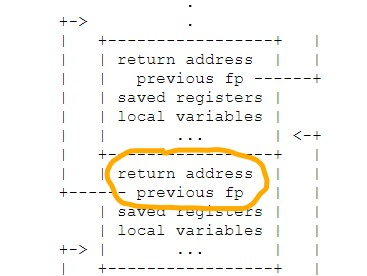
\includegraphics[height=4cm,width=5.3cm]{lab4-4.jpg}
\end{figure}
2.具体实现:\par
(1)首先是前期准备工作:包括在kernel/risv.h中添加函数r\_fp();在kernel/defs.h中需添加backtrace()的函数声明;在panic和sleep中添加函数backtrace()的调用。\par
(2)重点实现:在kernel/printf.c中实现backtrace()。根据思路对fp进行递归,*(fp-8)是ra,*(fp-16)是下一个fp;循环结束条件用到了提示中给出的PGROUNDUP(fp),因为栈是往上递归的。最后代码如下:
\begin{figure}[H]
    \centering
    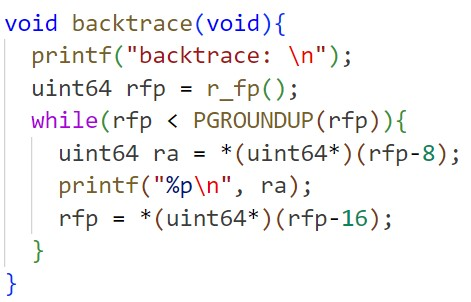
\includegraphics[height=4.5cm,width=5.7cm]{lab4-5.jpg}
\end{figure}
\newpage
\noindent 3.测试截图:
\begin{figure}[H]
    \centering
    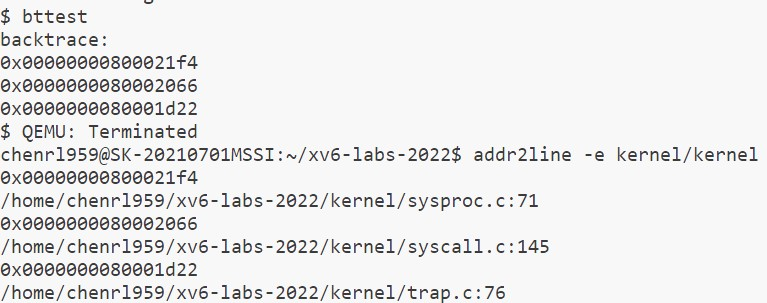
\includegraphics[height=4.5cm,width=8cm]{lab4-6.jpg}
\end{figure}
\begin{Large}
	\noindent 实验3-1:Alarm实验初步实现\\
\end{Large}
1.思路如下:\par
第一个部分里,sigreturn先直接返回0;重点在于sigalarm。修改后的proc应该能储存时间间隔、调用警报函数、已过去多少tick。这里重点在于对trap中usertrap的修改和sigalarm的实现。
根据提示,在usertrap中,若tick==interval,就清空tick并且跳转到目的函数,方法是修改trapframe->epc。\\
2.具体实现如下:\par
(1)完成准备工作,如添加系统调用、添加声明、完成简单的sigreturn函数(直接返回0)。\par
(2)完成对proc结构的修改,这里主要是间隔interval,函数指针handler,已过时间tick;并对proc.c中的allocproc进行修改,都初始化为0。\par
(3)完成对usertrap的修改,判interval是否为0$\rightarrow$判tick是不是达到标准$\rightarrow$修改p->trapframe->epc为handler。下面贴出代码,注释掉的是后面的。\par
(4)定义sigalarm,主要功能是通过argint argaddr读入参数,然后修改当前进程的interval/handler/tick。这之后已经能完成test0了,主要代码如下:
\begin{figure*}[!h]
    \centering
    \subfloat[in usertrap]{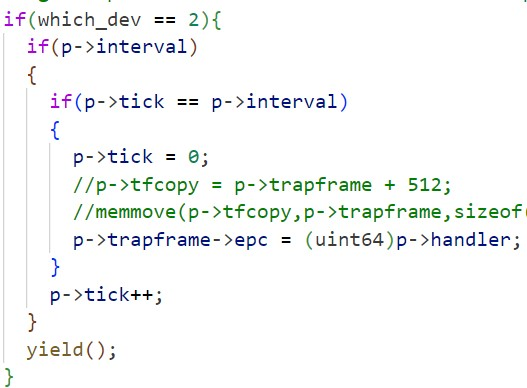
\includegraphics[width=6cm,height=5.5cm]{lab4-7.jpg} \label{X}}
    \hfill
    \subfloat[sigalarm]{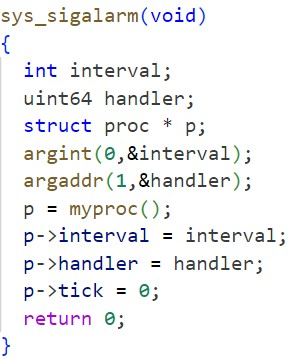
\includegraphics[width=4cm,height=6cm]{lab4-8.jpg} \label{Y}}
\end{figure*}
\newpage
\begin{Large}
	\noindent 实验3-2:Alarm实验进一步实现\\
\end{Large}
1.思路如下:\par
这里主要解决俩个问题,一个是寄存器的恢复与保存,还要避免重复alarm。第一个问题,我想到的解决方法是在改变epc前对信息进行备份,之后在sigreturn中拷贝回来即可,这需要proc中的补上新的字段,tfcopy。
第二个问题,我想到的简易解决是从tick出发;处于前面的设置,当且仅当tick==interval时才会触发,那么在触发后就让tick不置0,而是持续变大。\\
2.具体实现:\par
(1)完成struct proc和函数allocproc中的添加。\par
(2)修改usertrap,删去tick=0,并且在p->trapframe->epc更新前,将p->trapframe的内容拷贝给p->tfcopy(p->tfcopy初始被置为p->trapframe+512,(512?凑整+大于trapframe的288大小))。\par
(3)修改sigreturn,对p->tfcopy做判断,如果它是p->trapframe+512,那就进行恢复。最后要将tick,tfcopy置0。最后为了完成test3中对a0不能更改的要求,要返回p->trapframe->a0。代码如下:
\begin{figure*}[!h]
    \centering
    \subfloat[in usertrap]{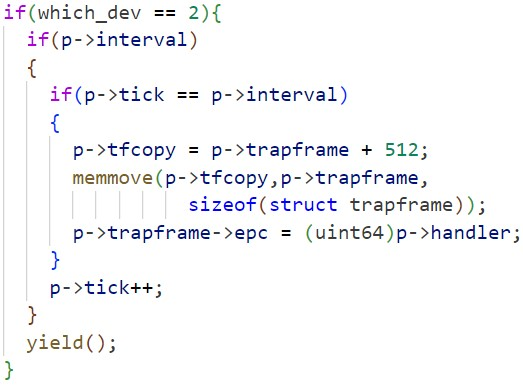
\includegraphics[width=5.5cm,height=6cm]{lab4-9.jpg} \label{X}}
    \hfill
    \subfloat[sigalarm]{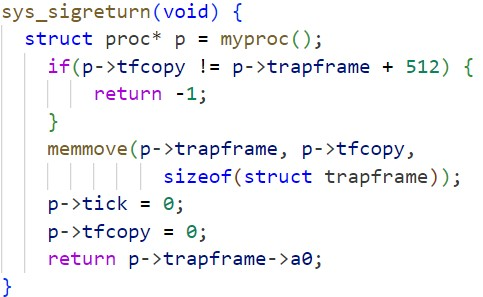
\includegraphics[width=5cm,height=5cm]{lab4-10.jpg} \label{Y}}
\end{figure*}\\
3.测试截图:
\begin{figure}[H]
    \centering
    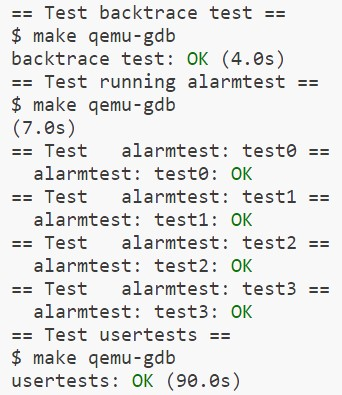
\includegraphics[height=5cm,width=3cm]{lab4-3.jpg}
\end{figure}
\end{document}